\documentclass[12pt]{article}
\usepackage[english]{babel}
\usepackage[letterpaper, left=1.0in,right=1.0in,top=1.0in,bottom=1.0in] {geometry}
\usepackage{booktabs}
\usepackage{caption}
\usepackage{subcaption}
\usepackage{amssymb,amsmath,amsfonts,breqn,titlesec,color,multirow,lscape,booktabs,setspace,eurosym,geometry,ulem,graphicx,caption,color,footmisc,caption,pdflscape,array,changepage}
\usepackage{graphicx}
\usepackage[colorlinks=true, allcolors=blue]{hyperref}
\renewcommand*\contentsname{Summary}


\begin{document}

\section{Histogram of construction investment}
Figure \ref{fig:hist1} shows construction value size in Billions of U.S. dollars at the state and year level.
\vspace*{\baselineskip}

\begin{figure}[hp]
    \centering
    \caption{Construction Value} 
    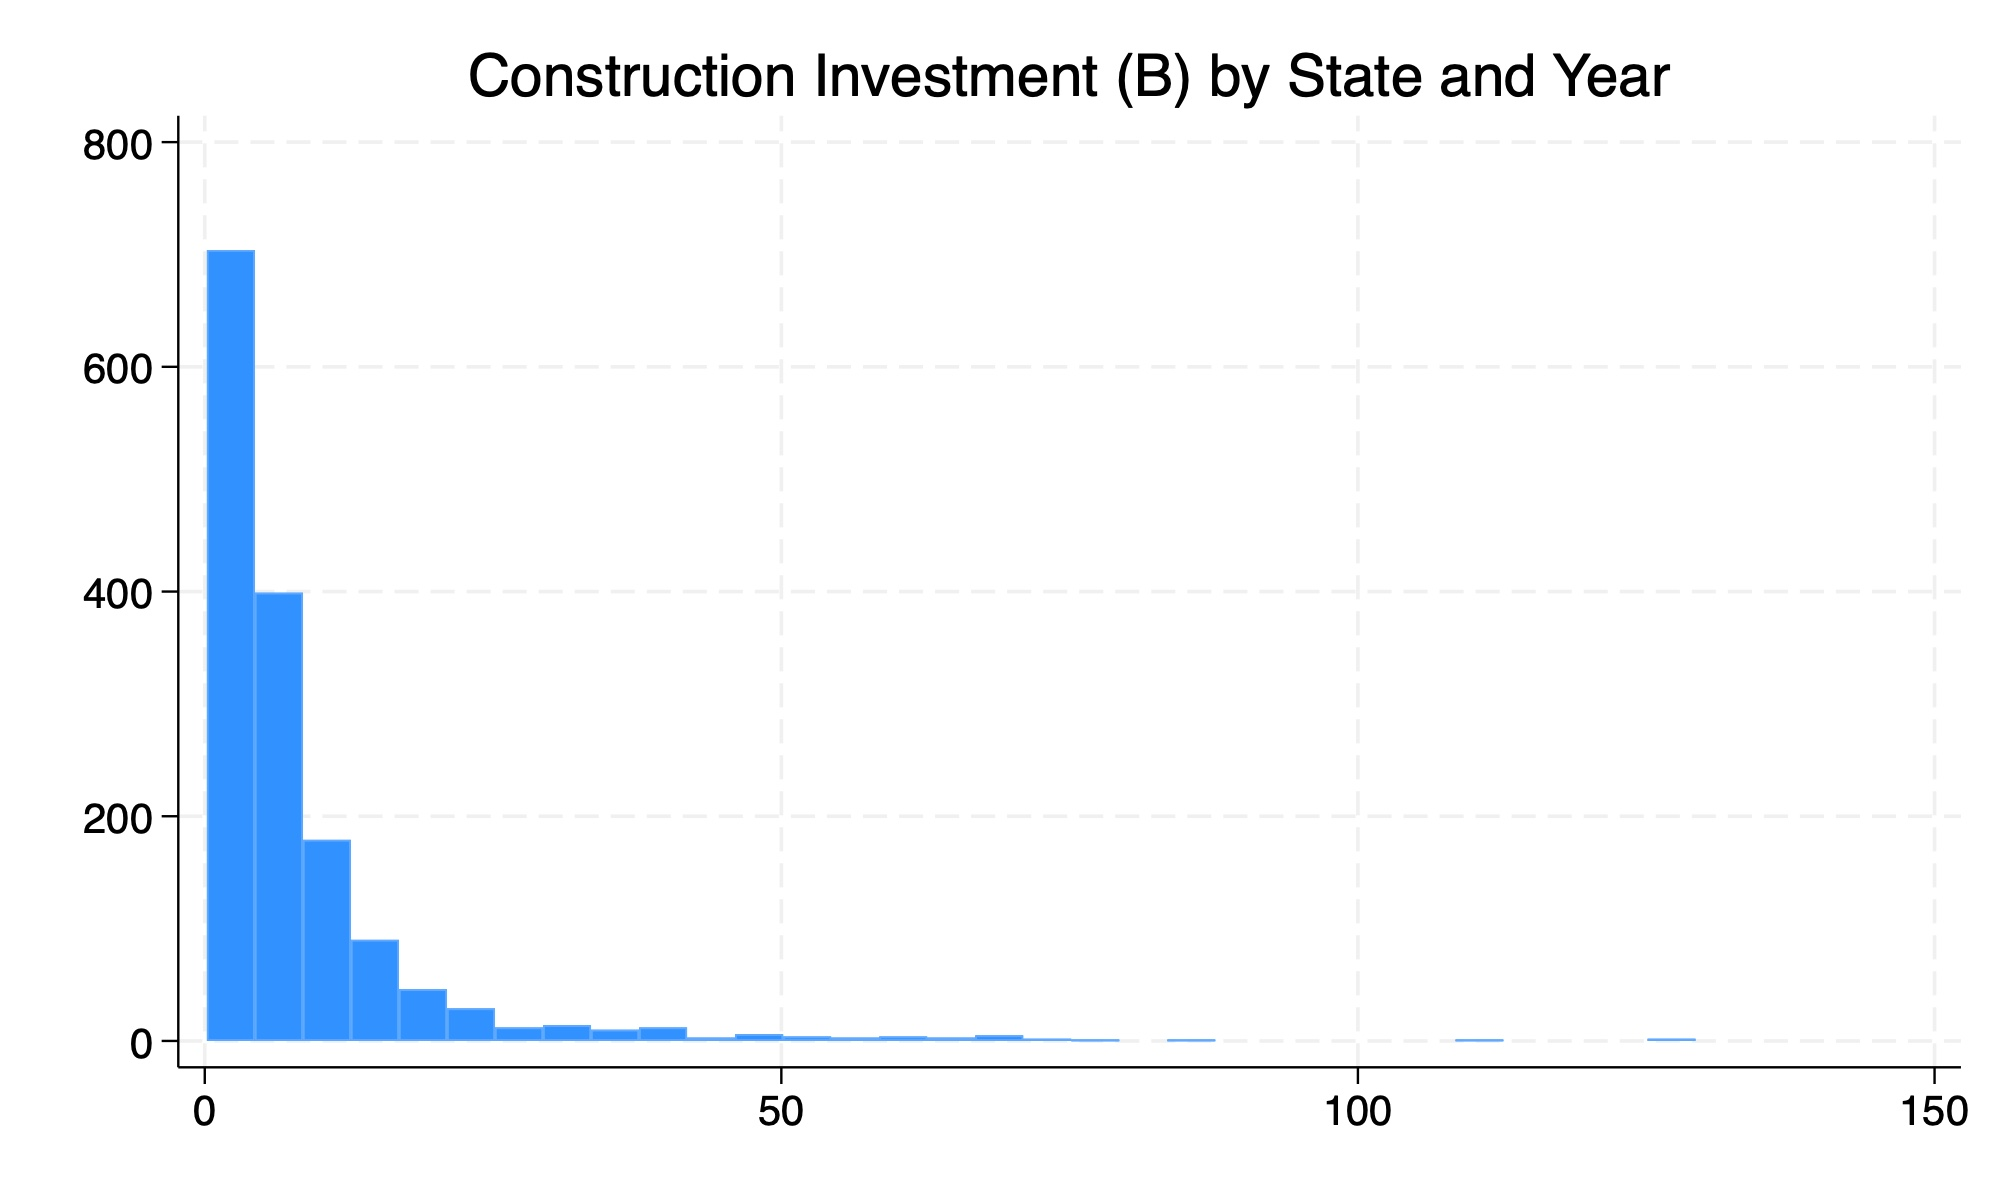
\includegraphics[width=0.9\textwidth]{histinv.jpg}
    \label{fig:hist1}
\end{figure}
    \begin{center} \vspace*{-\baselineskip}
        \footnotesize \singlespacing {Note: Including only projects with non-missing value information.}
    \end{center}


\end{document}